\documentclass[12pt,a4paper]{article}
\synctex=1
\usepackage[utf8]{inputenc}
\usepackage[margin=1cm]{geometry}
\usepackage{graphicx}
%\usepackage{verbatim}
\usepackage{listings}
\usepackage{textcomp}
\usepackage{courier}
\usepackage{libertine}
\usepackage{pgfornament}
\usepackage{eso-pic}
\usepackage{amsmath}
\usepackage[hangul]{kotex}
\linespread{1.3}

\title{
	\centering
	\pgfornament[width=12cm,color=teal]{84}\\
	\vspace{1cm}
	\fontsize{50}{50} \selectfont {
	3D Game Development\\Space War}
		\pgfornament[width=12cm,color=teal]{88}\\
	\vfill}
\author{
	\LARGE
	\begin{tabular}{rl}
		\hline
		학번 : & 2016110056\\ 
		학과 : & 불교학부 \\
		이름 : & 박승원\\
		날짜 : & \today\\
		\hline
	\end{tabular}\vspace{2cm}
	\\

\includegraphics[width=0.5\textwidth]{logo.jpg}
	}
\date{}


\begin{document}
\maketitle
\pagenumbering{gobble}
\noindent
\lstset{language=C++, columns=flexible, tabsize=4, frame=shadowbox, showstringspaces=false, breaklines=true, upquote=true, basicstyle=\normalsize}
\newpage
\section{Game Concept}
Destroy various enemies(space monkey, ironman, missile etc..) by maneuvering your spaceship.

\section{Control}
move with mouse, rotate ship with Q,E key

\section{Implementation}
Main class is GLObject(3D object) and GLObjs(a container of 3D objs).
First add 3D objects to container.
Then you can draw that object with index like GLObjs(0) which will draw the first object in the container.

I used threads and mutex to make play smoother.
\begin{lstlisting}
	objs += spaceship;
	objs += background;
	objs += ironman;
	objs += missile;
	objs += monkey;
	objs += hare;
	objs += dummy;
	objs += projectile;
	objs.transfer_all();


objs.matrix(proj * m.gltranslate(x,y,0) * m.glrotateZ(thz) * objs[0]);
objs(0);//spaceship
lock2.lock();
for(auto& a : enemies) {
	objs.matrix(proj * m.gltranslate(a[1][1],a[1][2],a[1][3]) * objs[a[1][4]]);
	objs(a[1][4]);//enemy
	a[1][3] += 0.05;//advance forward
}
lock2.unlock();
objs.matrix(proj * objs[1]);
objs(1);//background
	
lock1.lock();
for(auto& a : bullets) {
	objs.matrix(proj * a.time_pass() * objs[7]);
	objs(7);//bullet
}
lock1.unlock();
glfwSwapBuffers(window);
glfwPollEvents();

\end{lstlisting}

\section{Game Screen}
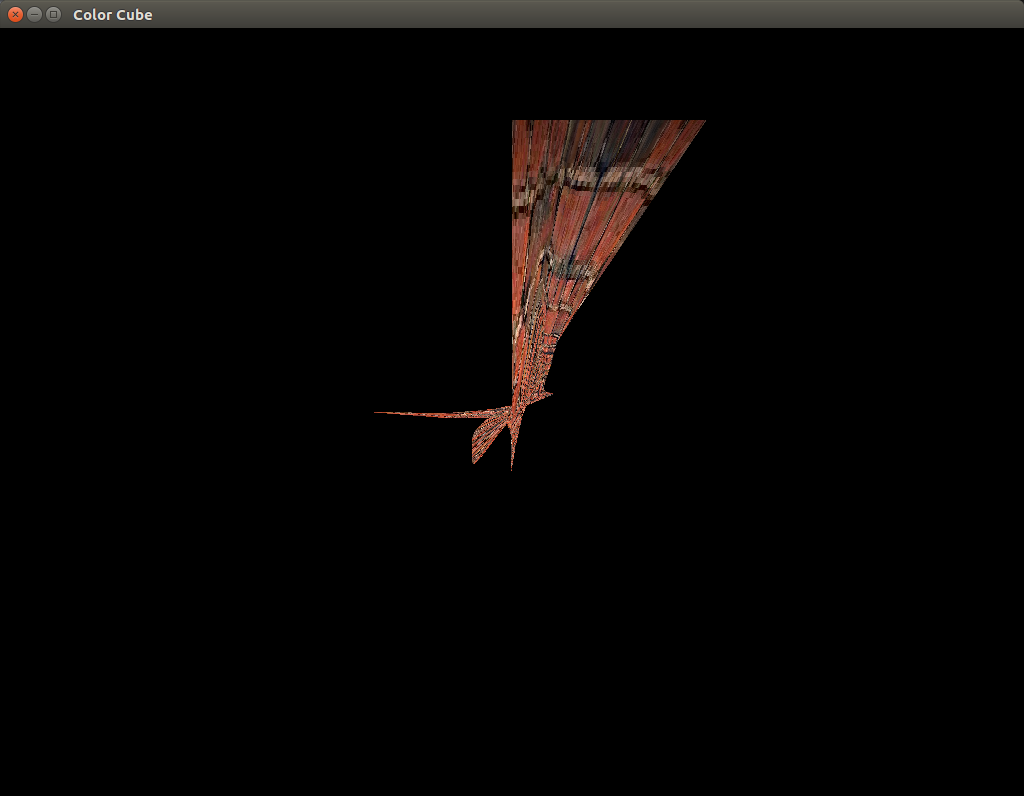
\includegraphics[width=\textwidth]{1.png}

\end{document}
